%%
%%     poster用 latex template
%%

%% platex -> dvipdfmx
\documentclass[36pt,twocolumn,dvipdfmx]{jsarticle}
%% optionにpapersize入れるとgeometryに怒られるので注意!

%% settings: paper size, margin
\usepackage[a0paper,truedimen]{geometry}
\geometry{
  margin = 3truecm % 周りの余白(margin)
}

%% FONT
\usepackage[T1]{fontenc} % font encoding を変更: OT1 → T1
\usepackage{lmodern} % Latin Modern フォントを使う
\usepackage[expert,deluxe]{otf} % font
% \renewcommand{\headfont}{\bfseries} % 見出しのフォント

%% 図
\usepackage[dvipdfmx]{graphicx} % 図の挿入
% \usepackage{wrapfig} % 文章中に図
\usepackage{here} % option H で図を強制出力

%% その他 sty
\usepackage{enumitem} % enumerate強化
\usepackage{url} % URLをそのまま表示してくれる
% \usepackage{ascmac} % 枠を作るやつ
\usepackage{xcolor} % 色を付ける
\usepackage{tikz} % おえかきできるツール

%% マクロ
\def\atag{\refstepcounter{equation}\tag{\theequation}}% 数式番号付加
\newcommand\QED{\hfill □\par} % put QED
\newcommand\siki[1]{(\ref{eq:#1})}
\newcommand\zu[1]{図\ref{fig:#1}}
\newcommand\hyo[1]{表\ref{tab:#1}}
\newcommand\ftj[1]{{\bfseries #1}}


%% - - - - - - - - - - - - - - - - - - - - -
\title{てんぷれタイトル}
\author{理工学部 物理科学科 4回生 \\ 中山 敦貴}
% \date{}
\date{\today}
% \date{令和元年12月1日}
%% - - - - - - - - - - - - - - - - - - - - -

\begin{document}%% - - - - - - - - - - - - -
%%
\maketitle % titleとか出力
\thispagestyle{empty}
%%

\section*{はじめに}
モチベとか概要とか書けばよいかと。

\section{なんちゃら}
ああああ

\section{おおおお?}
あああああああああああああああああああああああああ
ああああああああああああああああああああああああああ
あああああああああああああああああああああああああああ
ああああああああああああああああああああああああああああ

\section{です}
A0ポスターのtemplateです!
適当にググって作りました。
もっといい方法があったら教えてください。


%%
\newpage
\section{チートシート}

\subsection{figure環境}
図\ref{fig:sin}はイケメンです。
\begin{figure}[htbp]
  \centering
  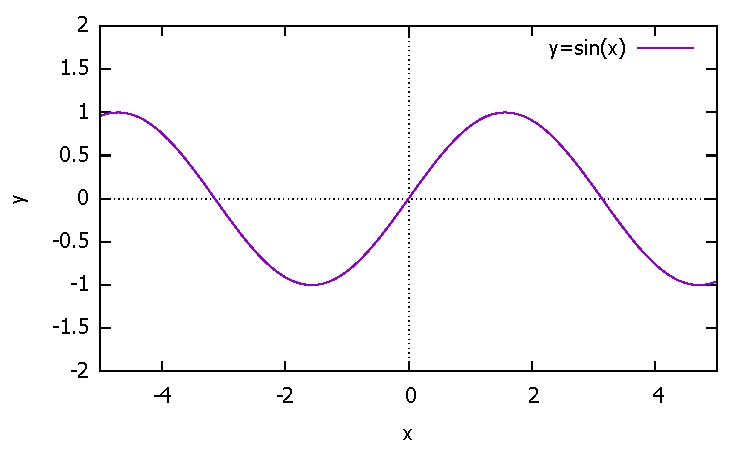
\includegraphics[width=.8\linewidth]{img/fig-sin.pdf}
  \caption{$y=\sin x$のグラフ。gnuplotで作成した。}
  \label{fig:sin}
\end{figure}

\subsection{table環境}
表\ref{tbl:vegetable}は僕の主観です。
\begin{table}[htbp]
  \centering
  \caption{やさいの表}
  \label{tbl:vegetable}
  \begin{tabular}{r|ccc} \hline
    No. & やさい & いろ & 印象 \\ \hline
    1 & トマト & あかいろ & くさい \\
    2 & キャベツ & みどり & 無味乾燥 \\
    3 & かぼちゃ & きいろ & かたい \\
    4 & にんじん & おれんじ & ゴミ \\ \hline
  \end{tabular}
\end{table}

%% 参考文献
\begin{thebibliography}{99}
  \item 著者1・著者2,『本のタイトル』,出版社,出版年.
  \item ページの著者,『ページのタイトル』,最終アクセス日,\\
    (\url{https://vuccaken.github.io}).
  % \bibitem{キー1} 著者,『本のタイトル』,出版社,出版年.
\end{thebibliography}




%%
% \end{multicols}
%%
\end{document}%% - - - - - - - - - - - - - -
%%
%% お疲れなのだ
%%